\documentclass[12pt]{report}
\usepackage[utf8]{inputenc}
\usepackage[T2A]{fontenc}
\usepackage[russian]{babel}
%\usepackage[14pt]{extsizes}
\usepackage{listings}
\usepackage{graphicx}
\usepackage{amsmath,amsfonts,amssymb,amsthm,mathtools}
\usepackage{pgfplots}
\usepackage{filecontents}
\usepackage{indentfirst}
\usepackage{eucal}
\usepackage{enumitem}
% Для \abs{}
\usepackage{commath}
\usepackage{float}
\frenchspacing


\usetikzlibrary{datavisualization}
\usetikzlibrary{datavisualization.formats.functions}

\usepackage[left=2cm,right=2cm, top=2cm,bottom=2cm,bindingoffset=0cm]{geometry}
% Для измененных титулов глав:
\usepackage{titlesec, blindtext, color} % подключаем нужные пакеты
\definecolor{gray75}{gray}{0.75} % определяем цвет
\newcommand{\hsp}{\hspace{20pt}} % длина линии в 20pt
% titleformat определяет стиль
\titleformat{\chapter}[hang]{\Huge\bfseries}{\thechapter\hsp\textcolor{gray75}{|}\hsp}{0pt}{\Huge\bfseries}

% plot
\usepackage{xcolor}
\usepackage{stmaryrd}
\usepackage{wasysym}
\usetikzlibrary{datavisualization}
\usetikzlibrary{datavisualization.formats.functions}

% листинги
\lstset{
    language = java,
    basicstyle=\small\sffamily,
    numbers=left,
    numberstyle=\tiny,
    stepnumber=1,
    numbersep=5pt,
    showspaces=false,
    showstringspaces=false,
    showtabs=false,
    frame=single,
    tabsize=2,
    captionpos=t,
    breaklines=true,
    breakatwhitespace=false,
    escapeinside={\#*}{*)}
}

\begin{document}
%\def\chaptername{} % убирает "Глава"
    % Титульник
    \thispagestyle{empty}
    \begin{titlepage}
        \noindent \begin{minipage}{0.15\textwidth}
                      
\includegraphics[width=\linewidth]{img/b_logo}
        \end{minipage}
        \noindent\begin{minipage}{0.9\textwidth}
                     \centering
                     \textbf{Министерство науки и высшего образования Российской Федерации}\\
                     \textbf{Федеральное государственное бюджетное образовательное учреждение высшего образования}\\
                     \textbf{~~~«Московский государственный технический университет имени Н.Э.~Баумана}\\
                     \textbf{(национальный исследовательский университет)»}\\
                     \textbf{(МГТУ им. Н.Э.~Баумана)}
        \end{minipage}

        \noindent\rule{18cm}{3pt}
        \newline\newline
        \noindent ФАКУЛЬТЕТ $\underline{\text{«Информатика и системы управления»}}$ \newline\newline
        \noindent КАФЕДРА $\underline{\text{«Программное обеспечение ЭВМ и информационные технологии»}}$\newline\newline\newline\newline\newline


        \begin{center}
            \noindent\begin{minipage}{1.3\textwidth}
                         \centering
                         \Large\textbf{  Отчет по лабораторной работе №1}\newline
                         \textbf{по дисциплине "Анализ алгоритмов"}\newline\newline
            \end{minipage}
        \end{center}

        \noindent\textbf{Тема} $\underline{\text{Расстояние Левенштейна}}$\newline\newline
        \noindent\textbf{Студент} $\underline{\text{Шацкий Р.Е.}}$\newline\newline
        \noindent\textbf{Группа} $\underline{\text{ИУ7-55Б}}$\newline\newline
        \noindent\textbf{Оценка (баллы)} $\underline{\text{~~~~~~~~~~~~~~~~~~~~~~~~~~~}}$\newline\newline
        \noindent\textbf{Преподаватели} $\underline{\text{Волкова Л.Л., Строганов Ю.В.}}$\newline\newline\newline

        \begin{center}
            \vfill
            Москва~---~\the\year
            ~г.
        \end{center}
    \end{titlepage}

    \tableofcontents

    % Введение
    \newpage
    \chapter*{Введение}
    \addcontentsline{toc}{chapter}{Введение}
    \textbf{Расстояние Левенштейна} --- минимальное количество операций вставки одного символа, удаления одного символа
    и замены одного символа на другой, необходимых для преобразования одной строки в другую.

    Ниже перечислены области применения расстояния Левенштейна в теории информации и компьютерной лингвистике.
%    Расстояние Левенштейна применяется в теории информации и компьютерной лингвистике для:
    \begin{itemize}
        \item исправления ошибок в слове;
        \item сравнения текстовых файлов утилитой diff;
        \item сравнения генов, хромосом и белков в биоинформатике.
    \end{itemize}

    Ниже перечислены цели лабораторной работы.
%    Цели лабораторной работы:
    \begin{enumerate}
        \item Изучить методы динамического программирования на основе алгоритмов нахождения расстояния
        Левенштейна и Дамерау-Левенштейна.
        \item Оценить реализации алгоритмов нахождения расстояния Левенштейна и Дамерау-Левенштейна.
    \end{enumerate}

    Ниже перечислены задачи лабораторной работы.
%    Задачи лабораторной работы:
    \begin{enumerate}
        \item Изучить принципы работы алгоритмов Левенштейна и Дамерау-Левенштейна.
        \item Подготовить тесты поиска расстояния между строками.
        \item Применить методы динамического программирования для матричной реализации указанных алгоритмов.
        \item Получить практические навыки реализации данных алгоритмов: итерационные и рекурсивные версии.
        \item Сравнить итерационные и рекурсивные реализации алгоритмов по затрачиваемым ресурсам (время и память).
        \item Получить экспериментальным методом различия во временной эффективности алгоритмов.
        \item Описать и обосновать полученные результаты в отчете о выполненной лабораторной работе
        в формате расчетно-пояснительной записки.
    \end{enumerate}

    % Аналитическая часть
    \newpage


    \chapter{Аналитическая часть}

    Расстояние Левенштейна~\cite{levenshtein} между двумя строками ---
    минимальное количество операций вставки одного символа, удаления одного символа
    и замены одного символа на другой, необходимых для преобразования одной строки в другую.

    Цена каждой операции может зависеть от вида операции или от участвующих в ней символов, отражающих вероятность
    разных ошибок при вводе текста.
    \\
    Далее рассмотрены виды операций и их цены.
    \begin{enumerate}
        \item Вставка (insert), $w(a,\lambda)$ --- цена удаления символа $a$.
        \item Удаление (delete), $w(\lambda, b)$ --- цена вставки символа $b$.
        \item Замена (replace), $w(a, b)$ --- цена замены символа $a$ на символ $b$.
    \end{enumerate}

    Для решения задачи о нахождении редакционного расстояния необходимо найти последовательность операций, при которых
    суммарная цена операций будет минимальной. Расстояние Левенштейна - частный случай решения этой задачи
    при перечисленных ниже условиях.
    \begin{itemize}
        \item $w(a, a) = 0$;
        \item $w(a, b) = 1, a \neq b$;
        \item $w(a, \lambda) = 1$;
        \item $w(\lambda, b) = 1$.
    \end{itemize}


    \section{Рекурсивный алгоритм нахождения расстояния Левенштейна}\label{sec:ReccursiveLev}
    В основе вычисления расстояние Левенштейна между двумя строками a и b лежит формула~\ref{eq:D}.
    При описании алгоритмов и формул будут использоваться указанные ниже обозначения.
    \begin{itemize}
        \item $\abs{a}$ --- длина строки $a$;
        \item $a[i]$ --- \emph{i}-ый символ строки $a$.
    \end{itemize}

    \begin{equation}
        \label{eq:D}
        D(i, j) = \begin{cases}
                      0 &\text{i = 0, j = 0} \\
                      i &\text{j = 0, i > 0} \\
                      j &\text{i = 0, j >0} \\
                      \min \lbrace \\
                      \qquad D(i, j - 1) + 1 \\
                      \qquad D(i - 1, j) + 1 &\text{i > 0, j > 0} \\
                      \qquad D(i - 1, j - 1) + m(a[i], b[j]) &\text{\ref{eq:m}} \\
                      \rbrace
        \end{cases}
    \end{equation}

    Функция~\ref{eq:m} позволяет сравнить два символа:
    \begin{equation}
        \label{eq:m}
        m(a, b) = \begin{cases}
                      0 &\text{a = b} \\
                      1 &\text{иначе}
        \end{cases}
    \end{equation}

    Рекурсивный алгоритм реализует формулу~\ref{eq:D}.
    Логика функции $D$ описана ниже.
    \begin{enumerate}
        \item Для получения из пустой строки пустой строки, требуется 0 операций.
        \item Для получения из пустой строки строки $b$ требуется \abs{b} операций (все - insert).
        \item Для получения из строки $a$ пустой строки требуется \abs{a} операций (все - delete).
        \item Для получения из строки $a$ строки $b$ требуется выполнить несколько операций.
        Обозначая $a'$ и $b'$ за строки $a$ и $b$ без последнего символа соответсвенно, цену преобразования
        из строки $a$ в $b$ можно выразить следующим образом:
        \begin{enumerate}
            \item Сумма цены преобразования строки $a'$ в $b$ и цены операции удаления (для преобразования $a'$ в $a$)
            \item Сумма цены преобразования строки $a$ в $b'$ и цены операции вставки (для преобразования $b'$ в $b$)
            \item Сумма цены преобразования строки $a'$ в $b'$ и операции замены
            (если a и b оканчиваются на разные символы)
            \item Цена преобразования строки $a'$ в $b'$ (если $a$ и $b$ оканчиваются на одинаковый символ)
        \end{enumerate}
        Минимальная цена преобразования --- минимальное значение из приведенных выше вариантов.
    \end{enumerate}


    \section{Итерационный алгоритм нахождения расстояния Левенштейна с использованием матрицы}
    Прямая реализация формулы~\ref{eq:D} может быть неэффективна при больших значениях длин строк,
    поскольку промежуточные значения функции $D(i, j)$ вычисляются несколько раз.
    Для оптимизации алгоритма можно использовать матрицу для хранения промежуточных значений функции $D(i, j)$.
    В таком случае алгоритм выполняет построчное заполнение матрицы, пока не дойдет до крайнего правого элемента,
    в котором будет записано итоговое расстояние Левенштейна.


    \section{Рекурсивный алгоритм нахождения расстояния Левенштейна с использованием матрицы}
    Основной недостаток обычного рекурсивного алгоритма --- многократное вычисления промежуточных значений
    функции D(i, j).
    Этот недостаток можно устранить, и сделать таким образом алгоритм более эффективным по времени выполнения,
    если добавить матрицу, которая будет заполняться промежуточными значениями D(i, j).
    Если рекурсивный алгоритм обрабатывает данные, которые еще ни разу не были поданы, результат
    записывается в матрицу.
    Если рекурсивный алгоритм обрабатывает данные, которые уже были обработаны, берется старый результат из матрицы.


    \section{Расстояние Дамерау-Левенштейна}
    Расстояние Дамерау-Левенштейна очень похоже на расстояние Левенштейна, но в его поиске используется еще одна
    операция - \textbf{транспозиция} (перестановка двух соседних символов).

    Расстояние Дамерау-Левенштейна между двумя строками a и b определяется функцией~\ref{eq:dl}:

    \begin{equation}
        \label{eq:dl}
        d_{a, b}(i, j) =
        \begin{cases}
            \max(i, j)
            & \text{если } \min(i, j) = 0
            \\
            \min
            \begin{cases}
                d_{a, b}(i - 1, j) + 1
                \\
                d_{a, b}(i, j - 1) + 1
                \\
                d_{a, b}(i - 1, j - 1) + m(a[i], b[j])
                \\
                d_{a, b}(i - 2, j - 2) + 1
            \end{cases}
            & \begin{aligned}
                  \text{если } i, j > 1 \\ \text{и } a[i] = b[j - 1] \\ \text{ и } a[i - 1] = b[j]
            \end{aligned}
            \\
            \min
            \begin{cases}
                d_{a, b}(i - 1, j) + 1
                \\
                d_{a, b}(i, j - 1) + 1
                \\
                d_{a, b}(i - 1, j - 1) + m(a[i], b[j])
            \end{cases}
            & \text{иначе}
            \\
        \end{cases}
    \end{equation}
    Формула выводится по тем же соображениям, что и~\ref{eq:D}. Прямое применение рекурсивной функции тоже
    неэффективно по времени исполнения, так что аналогично методу, описанному в~\ref{sec:ReccursiveLev}
    добавляется матрица для хранения промежуточных значений.


    \section{Вывод}
    В данном разделе были рассмотрены алгоритмы нахождения расстояния Левенштейна и Дамерау-Левенштейна.
    Формулы Левенштейна и Дамерау-Левенштейна для нахождения расстояния между строками задаются рекурсивно
    и программно могут быть реализованы как рекурсивно, так и итерационно.

    \newpage


    \chapter{Конструкторская часть}


    \section{Разработка алгоритмов}
    В данной части будут рассмотрены схемы алгоритмов нахождения расстояния Левенштейна и Дамерау-Левенштейна.
    На рисунках~\ref{fig:levRecur} -~\ref{fig:levDamCasual2} представлены рассматриваемые алгоритмы

    \begin{figure}[H]
        \centering
        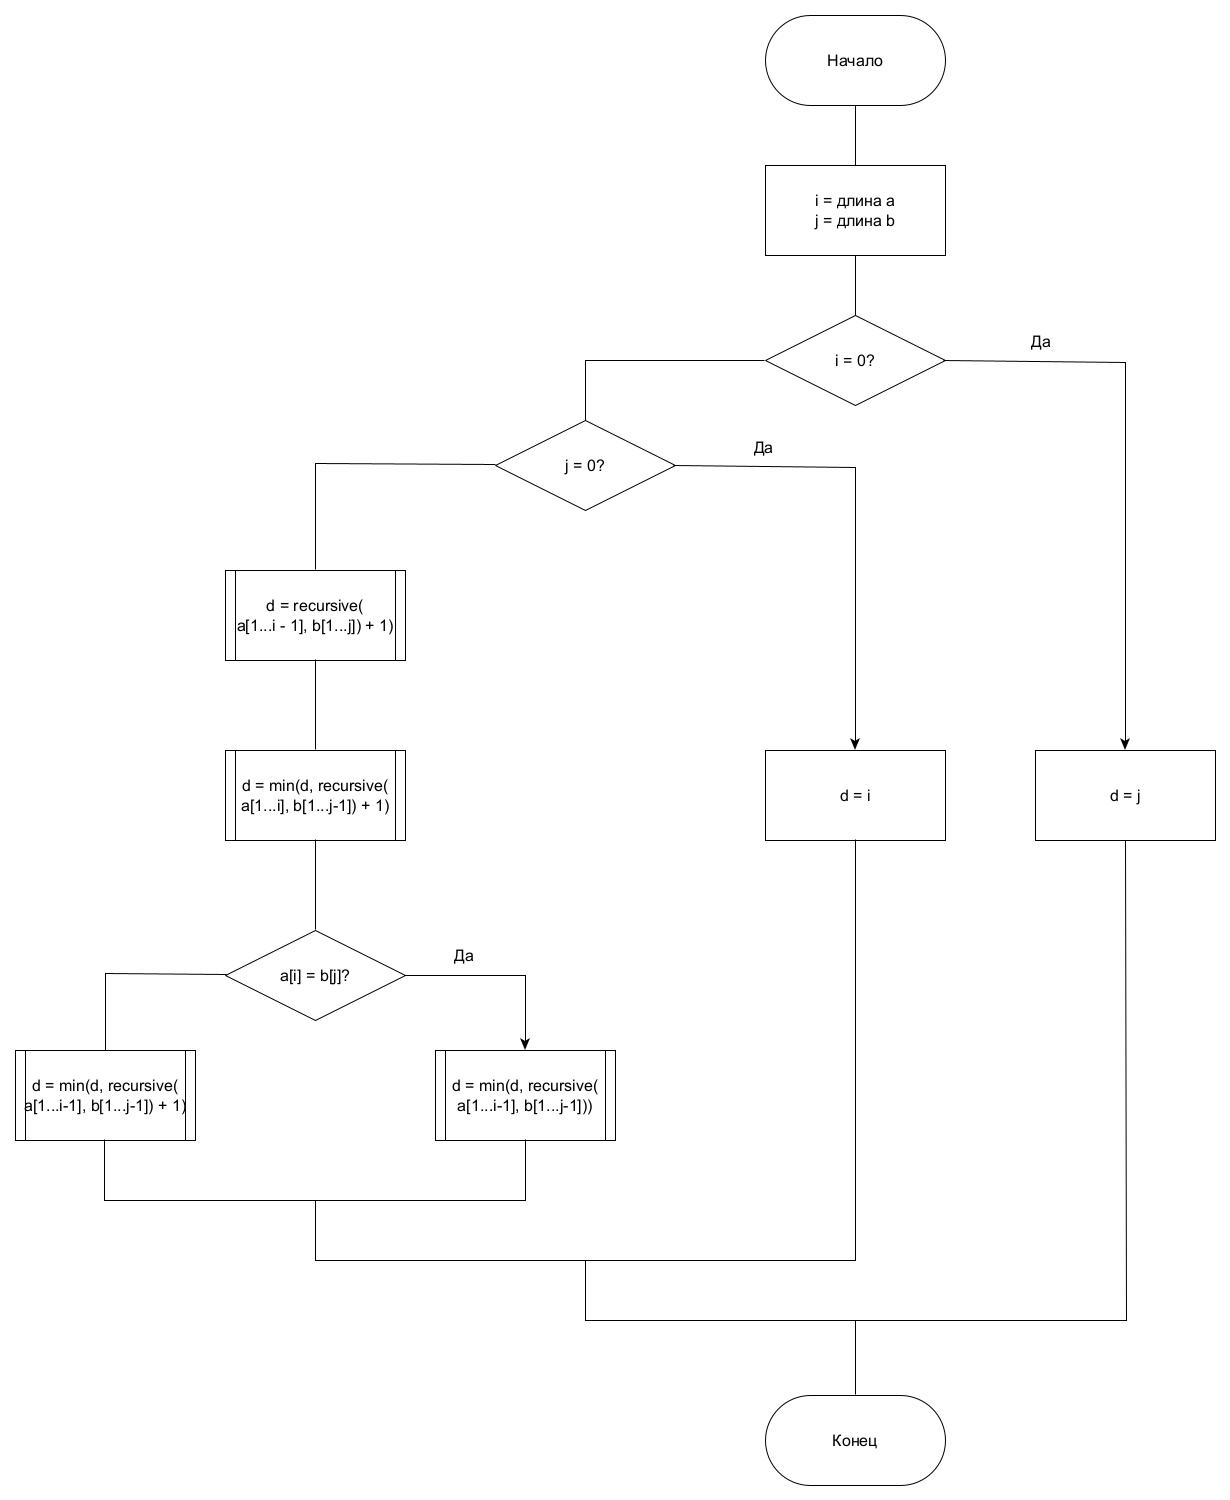
\includegraphics[width=1\linewidth]{img/levRecur}
        \caption{\begin{center}
                     Блок-схема рекурсивного агоритма нахождения расстояния Левенштейна
        \end{center}}
        \label{fig:levRecur}
    \end{figure}

    \begin{figure}[H]
        \centering
        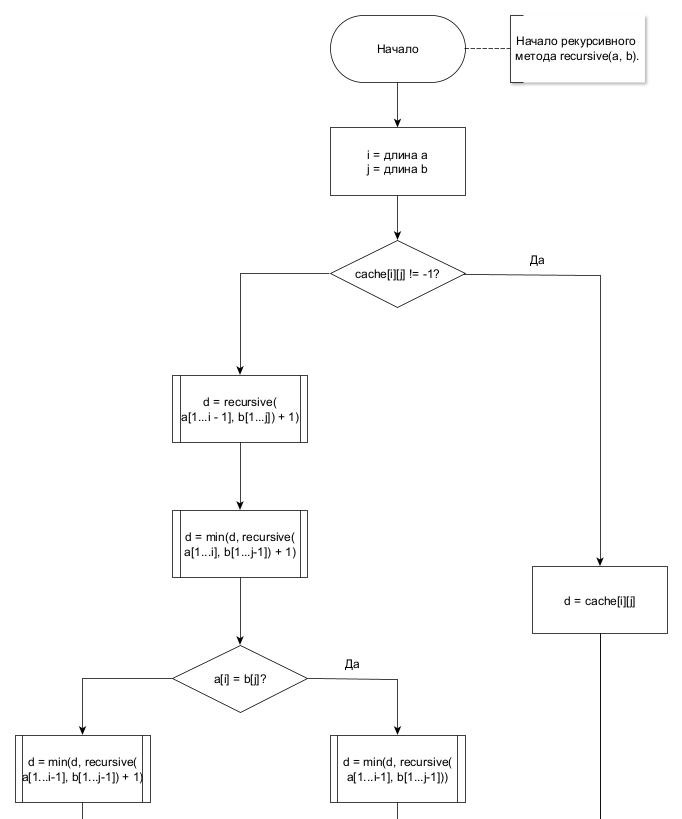
\includegraphics[width=1\linewidth]{img/levRecurCache1}
        \caption{\begin{center}
                     Блок-схема рекурсивного алгоритма нахождения расстояния Левенштейна с использованием матрицы ч.1
        \end{center}}
        \label{fig:levRecurCache1}
    \end{figure}

    \begin{figure}[H]
        \centering
        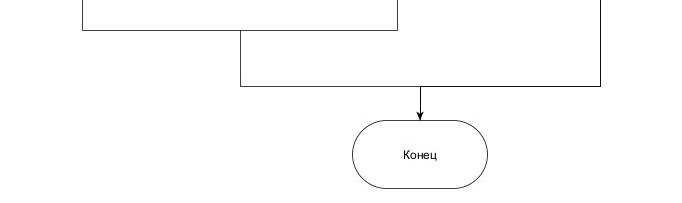
\includegraphics[width=1\linewidth]{img/levRecurCache2}
        \caption{
            \begin{center}
                Блок-схема рекурсивного алгоритма нахождения расстояния Левенштейна с использованием матрицы ч.2
            \end{center}}
        \label{fig:levRecurCache2}
    \end{figure}


    \begin{figure}[H]
        \centering
        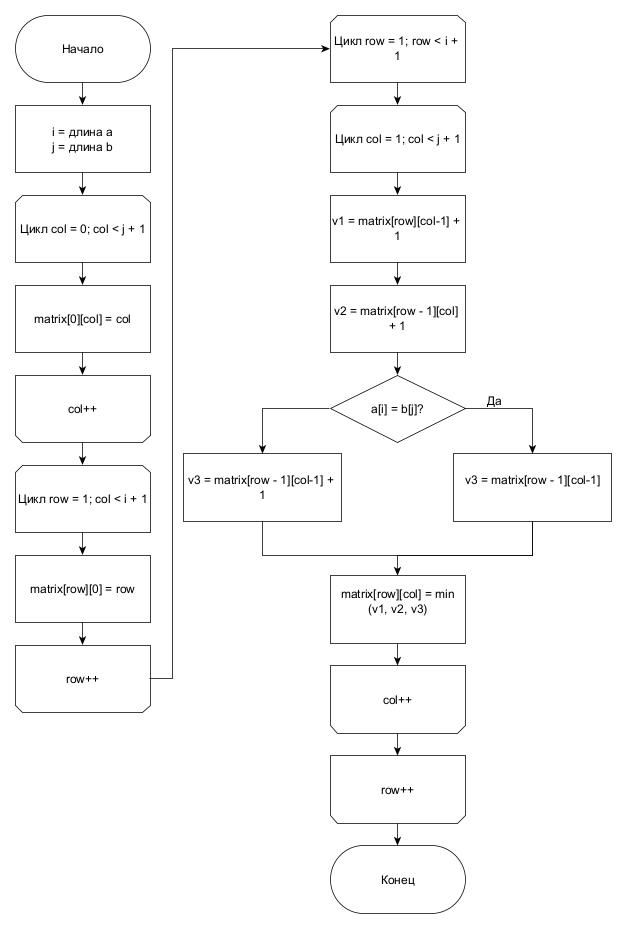
\includegraphics[width=0.85\linewidth]{img/levCasual}
        \caption{
            \begin{center}
                Блок-схема итерационного агоритма нахождения расстояния Левенштейна
            \end{center}}
        \label{fig:levCasual}
    \end{figure}


    \begin{figure}[H]
        \centering
        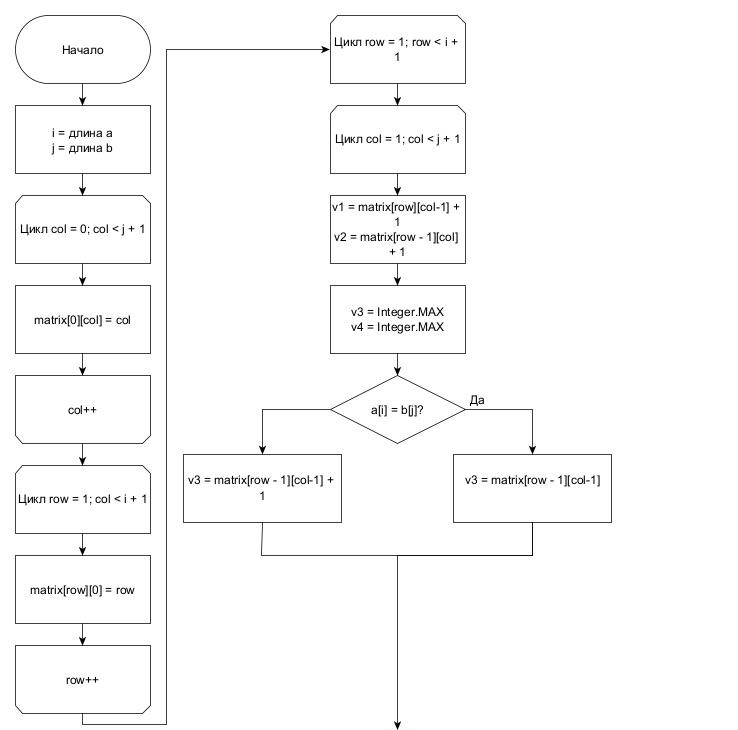
\includegraphics[width=1\linewidth]{img/levDamCasual1}
        \caption{
            \begin{center}
                Блок-схема итерационного агоритма нахождения расстояния Дамерау-Левенштейна ч.1
            \end{center}}
        \label{fig:levDamCasual1}
    \end{figure}

    \begin{figure}[H]
        \centering
        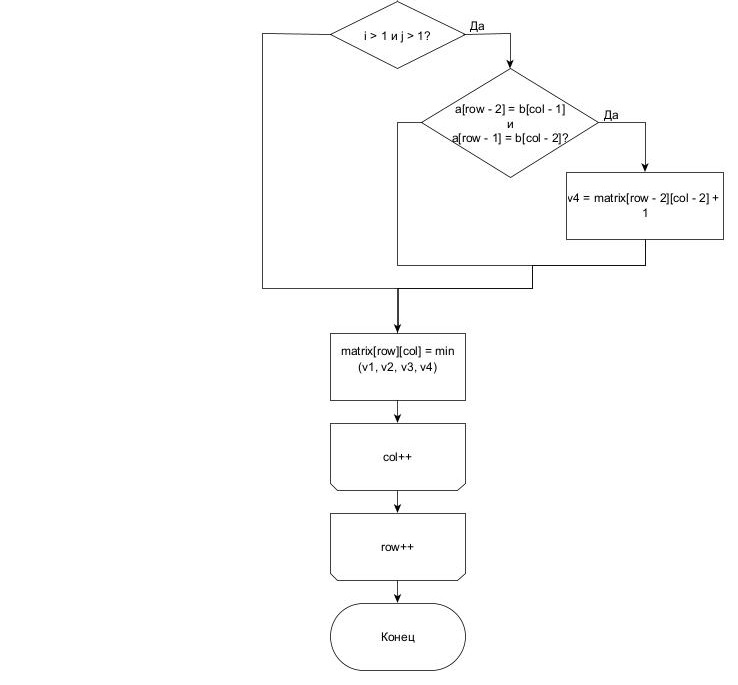
\includegraphics[width=1\linewidth]{img/levDamCasual2}
        \caption{
            \begin{center}
                Блок-схема итерационного агоритма нахождения расстояния Дамерау-Левенштейна ч.2
            \end{center}}
        \label{fig:levDamCasual2}
    \end{figure}


    \section{Вывод}
    На основе теоретических данных, полученных в аналитическом разделе,
    были построены блок-схемы исследуемых алгоритмов.


    \chapter{Технологическая часть}


    \section{Требование к ПО}
    Ниже перечислены основные требования к разрабатываемому ПО.
    \begin{enumerate}
        \item Предусмотреть возможность строк для сравнения и вывода результата сравнения;
        \item ПО должно выводить количество использованного процессорного времени;
        \item ПО должно работать корректно.
    \end{enumerate}


    \section{Средства реализации}
    Для реализации программы нахождения расстояния Левенштейна и Дамерау-Левенштейна
    был выбрал язык программирования Java~\cite{java}. Такой выбор обусловлен желанием
    расширить знания в области применения данного языка программирования.


    \section{Реализация алгоритмов}
    В листингах \ref{code:levrecur} - \ref{code:levDamCasual}
    приведена реализация алгоритмов нахождения расстояния Левенштейна и Дамерау-Левенштейна.

    \begin{lstlisting}[label={code:levrecur},caption=Метод для нахождения расстояния Левенштейна рекурсивно,
        language=java]
public class LevRecursion extends StringDistanceAlgorithm {
    public LevRecursion(String a, String b) {
        super(a, b);
    }

    public int findDifference() {
        return findDifference(a, a.length(), b, b.length());
    }

    private int findDifference(String a, int aLen, String b, int bLen) {
        if (aLen == 0) {
            return bLen;
        }
        if (bLen == 0) {
            return aLen;
        }

        int deletion = findDifference(a, aLen - 1, b, bLen) + 1;
        int insertion = findDifference(a, aLen, b, bLen - 1) + 1;

        int match = Objects.equals(a.charAt(aLen - 1), b.charAt(bLen - 1)) ? 0 : 1;
        int substitution = findDifference(a, aLen - 1, b, bLen - 1) + match;

        return Math.min(substitution, Math.min(deletion, insertion));
    }
}
    \end{lstlisting}

    \begin{lstlisting}[label=code:levRecurMatrix,caption=Метод для нахождения расстояния Левенштейна рекурсивно
    \(\text{с матрицей}\),language=java]
public class LevRecursionCache extends StringDistanceAlgorithm {
    int[][] cache;

    public LevRecursionCache(String a, String b) {
        super(a, b);
    }

    public int findDifference() {
        cache = new int[a.length() + 1][b.length() + 1];
        for (int[] a : cache) {
            Arrays.fill(a, -1);
        }

        return findDifference(a, a.length(), b, b.length());
    }

    private int findDifference(String a, int aLen, String b, int bLen) {
        if (cache[aLen][bLen] != - 1) {
            return cache[aLen][bLen];
        }
        if (aLen == 0) {
            return bLen;
        }
        if (bLen == 0) {
            return aLen;
        }

        int deletion = findDifference(a, aLen - 1, b, bLen) + 1;
        int insertion = findDifference(a, aLen, b, bLen - 1) + 1;

        int match = Objects.equals(a.charAt(aLen - 1), b.charAt(bLen - 1)) ? 0 : 1;
        int substitution = findDifference(a, aLen - 1, b, bLen - 1) + match;

        int min = Math.min(substitution, Math.min(deletion, insertion));
        cache[aLen][bLen] = min;
        return min;
    }
}
    \end{lstlisting}

    \begin{lstlisting}[label=code:levСasualMatrix,caption=Метод для нахождения расстояния Левенштейна итерационно,
        language=java]
public class LevCasualMatrix extends StringDistanceAlgorithm {
    private final int[][] matrix;

    public LevCasualMatrix(String a, String b) {
        super(a, b);
        matrix = new int[a.length() + 1][b.length() + 1];
    }

    public int findDifference() {
        for (int col = 0; col < matrix[0].length; col++) {
            matrix[0][col] = col;
        }

        for (int row = 1; row < matrix.length; row++) {
            matrix[row][0] = row;
        }

        for (int row = 1; row < matrix.length; row++) {
            for (int col = 1; col < matrix[0].length; col++) {
                int valueFromTheRight = matrix[row][col - 1] + 1;
                int valueFromTheUp = matrix[row - 1][col] + 1;

                int match = Objects.equals(a.charAt(row - 1), b.charAt(col - 1)) ? 0 : 1;
                int valueFromDiagonal = matrix[row - 1][col - 1] + match;

                matrix[row][col] = Math.min(valueFromTheRight, Math.min(valueFromTheUp, valueFromDiagonal));
            }
        }

        return matrix[a.length()][b.length()];
    }
}
    \end{lstlisting}

    \begin{lstlisting}[label=code:levDamRecursion,caption=Метод для нахождения расстояния Дамерау-Левенштейна
    рекурсивно,language=java]
public class LevDamRecursion extends StringDistanceAlgorithm {
    public LevDamRecursion(String a, String b) {
        super(a, b);
    }

    public int findDifference() {
        return findDifference(a, a.length(), b, b.length());
    }

    private int findDifference(String a, int aLen, String b, int bLen) {
        if (aLen == 0) {
            return bLen;
        }
        if (bLen == 0) {
            return aLen;
        }

        int deletion = findDifference(a, aLen - 1, b, bLen) + 1;
        int insertion = findDifference(a, aLen, b, bLen - 1) + 1;

        int match = Objects.equals(a.charAt(aLen - 1), b.charAt(bLen - 1)) ? 0 : 1;
        int substitution = findDifference(a, aLen - 1, b, bLen - 1) + match;

        int swap = Integer.MAX_VALUE;
        if (aLen > 1 && bLen > 1) {
            if (Objects.equals(a.charAt(aLen - 1), b.charAt(bLen - 2)) &&
                    Objects.equals(a.charAt(aLen - 2), b.charAt(bLen - 1))) {
                swap = findDifference(a, aLen - 2, b, bLen - 2) + 1;
            }
        }

        return Math.min(Math.min(swap, substitution), Math.min(deletion, insertion));
    }
}
    \end{lstlisting}

    \begin{lstlisting}[label=code:levDamRecursionCache,caption=Метод для нахождения расстояния Дамерау-Левенштейна
    рекурсивно \(\text{с матрицей}\),language=java]
public class LevDamRecursionCache extends StringDistanceAlgorithm {
    private int[][] cache;

    public LevDamRecursionCache(String a, String b) {
        super(a, b);
    }

    public int findDifference() {
        cache = new int[a.length() + 1][b.length() + 1];
        for (int[] a : cache) {
            Arrays.fill(a, -1);
        }

        return findDifference(a, a.length(), b, b.length());
    }

    private int findDifference(String a, int aLen, String b, int bLen) {
        if (cache[aLen][bLen] != -1) {
            return cache[aLen][bLen];
        }
        if (aLen == 0) {
            return bLen;
        }
        if (bLen == 0) {
            return aLen;
        }

        int deletion = findDifference(a, aLen - 1, b, bLen) + 1;
        int insertion = findDifference(a, aLen, b, bLen - 1) + 1;

        int match = Objects.equals(a.charAt(aLen - 1), b.charAt(bLen - 1)) ? 0 : 1;
        int substitution = findDifference(a, aLen - 1, b, bLen - 1) + match;

        int swap = Integer.MAX_VALUE;
        if (aLen > 1 && bLen > 1) {
            if (Objects.equals(a.charAt(aLen - 1), b.charAt(bLen - 2)) &&
                    Objects.equals(a.charAt(aLen - 2), b.charAt(bLen - 1))) {
                swap = findDifference(a, aLen - 2, b, bLen - 2) + 1;
            }
        }

        int min = Math.min(Math.min(swap, substitution), Math.min(deletion, insertion));
        cache[aLen][bLen] = min;
        return min;
    }
}
    \end{lstlisting}

    \begin{lstlisting}[label=code:levDamCasual,caption=Метод для нахождения расстояния Дамерау-Левенштейна
    итерационно,language=java]
public class LevDamCasualMatrix extends StringDistanceAlgorithm {
    private int[][] matrix;

    public LevDamCasualMatrix(String a, String b) {
        super(a, b);
        matrix = new int[a.length() + 1][b.length() + 1];
    }

    public int findDifference() {

        for (int col = 0; col < matrix[0].length; col++) {
            matrix[0][col] = col;
        }

        for (int row = 1; row < matrix.length; row++) {
            matrix[row][0] = row;
        }

        for (int row = 1; row < matrix.length; row++) {
            for (int col = 1; col < matrix[0].length; col++) {
                int valueFromTheRight = matrix[row][col - 1] + 1;
                int valueFromTheUp = matrix[row - 1][col] + 1;

                int match = Objects.equals(a.charAt(row - 1), b.charAt(col - 1)) ? 0 : 1;
                int valueFromDiagonal = matrix[row - 1][col - 1] + match;

                matrix[row][col] = Math.min(valueFromTheRight, Math.min(valueFromTheUp, valueFromDiagonal));

                int swap = Integer.MAX_VALUE;
                if (row > 1 && col > 1) {
                    if (Objects.equals(a.charAt(row - 1), b.charAt(col - 2)) &&
                            Objects.equals(a.charAt(row - 2), b.charAt(col - 1))) {
                        swap = matrix[row - 2][col - 2] + 1;
                    }
                }

                matrix[row][col] = Math.min(Math.min(valueFromTheRight, valueFromTheUp),
                        Math.min(swap, valueFromDiagonal));
            }
        }

        return matrix[a.length()][b.length()];
    }
}
    \end{lstlisting}


    \section{Тестовые данные}
    В таблице~\ref{tab:tests} приведены тестовые данные, на которых было протестировано разработанное ПО.
    Тестирование проводится по методу черного ящика.

    Все тесты были успешно пройдены

    \begin{table}[H]
        \centering
        \caption{Тестовые данные}
        \label{tab:tests}
        \begin{tabular}{|c c c c c|}
            \hline
            № & Первое слово & Второе слово & Ожидаемый результат & Полученный результат \\ [0.8ex]
            \hline
            1 & kot          & skat         & 2, 2                & 2, 2                 \\
            \hline
            2 & solution     & slouiton     & 4, 2                & 4, 2                 \\
            \hline
            3 & fumo         & mofu         & 4, 4                & 4, 4                 \\
            \hline
            4 &              &              & 0, 0                & 0,0                  \\
            \hline
            5 &              & aoa          & 3, 3                & 3, 3                 \\
            \hline
            6 & aoa          &              & 3, 3                & 3, 3                 \\
            \hline
            7 & текст        & ткскт        & 3, 2                & 3, 2                 \\
            \hline
        \end{tabular}
    \end{table}


    \section{Вывод}
    В данном разделе были разработаны исходные коды шести алгоритмов: вычисления расстояния
    Левенштейна и Дамерау-Левенштейна рекурсивно, рекурсивно с матрицей и итерационно


    \chapter{Исследовательская часть}


    \section{Пример работы программы}
    Демонстрация работы программы приведена на рисунке \ref{fig:workSample}

    \begin{figure}[H]
        \centering
        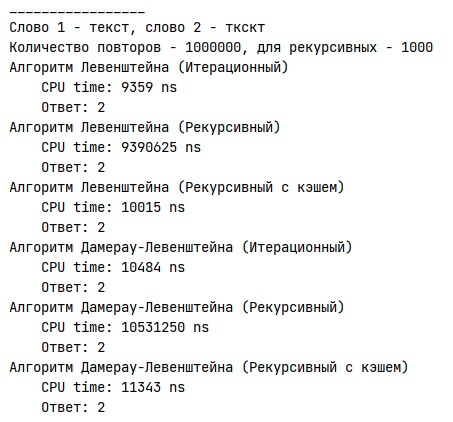
\includegraphics[scale=1]{img/workSample}
        \caption{Демонстрация работы программы}
        \label{fig:workSample}
    \end{figure}


    \section{Технические характеристики}
    Ниже приведены технические характеристики устройства, на котором были проведены замеры времени.
    \begin{itemize}
        \item операционная система --- Windows~\cite{windows} 10 64-bit;
        \item оперативная память --- 4 GB (для Java);
        \item процессор --- Intel(R) Core(TM) i5-7600 CPU @ 3.50GHz \cite{i5}.
    \end{itemize}


    \section{Время выполнения алгоритма}
    Время выполнения алгоритмов замерялось с помощью Java-интерфейса для управления потоками
    виртуальной машины Java - ThreadMXBean~\cite{threadMXBean}, позволяющего вычислить процессорное время,
    затраченное на определенный процесс.
    Процессорное время находилось как среднее арифметическое
    из нескольких разовых замеров процессорного времени (1000000 замеров).

    В таблице~\ref{tab:times} представлены замеры времени работы для каждого из алгоритмов.
    Сокращенные названия алгоритмов приведены ниже.
    \begin{itemize}
        \item Л-И --- Расстояние Левенштейна, итерационный алгоритм;
        \item Л-Р --- Расстояние Левенштейна, рекурсивный алгоритм;
        \item Л-Р-М --- Расстояние Левенштейна, рекурсивный алгоритм с использованием матрицы;
        \item ЛД-И --- Расстояние Дамерау-Левенштейна, итерационный алгоритм;
        \item ЛД-Р --- Расстояние Дамерау-Левенштейна, рекурсивный алгоритм;
        \item ЛД-Р-М --- Расстояние Дамерау-Левенштейна, рекурсивный алгоритм с использованием матрицы.
    \end{itemize}

    \begin{table}[H]
        \caption{Таблица времени выполнения алгоритмов (в наносекундах)}
        \label{tab:times}
        \centering
        \begin{tabular}{|c c c c c c c|}
            \hline
            Длина строк & Л-И   & Л-Р      & Л-Р-М  & ЛД-И   & ЛД-Р      & ЛД-Р-М \\
            \hline
            10          & 750   & 41718750 & 2500   & 3570   & 112187500 & 6125   \\
            \hline
            20          & 3156  & ---      & 8406   & 14906  & ---       & 22734  \\
            \hline
            50          & 17500 & ---      & 45264  & 89218  & ---       & 139843 \\
            \hline
            100         & 67656 & ---      & 193593 & 356562 & ---       & 546875 \\
            \hline
        \end{tabular}
    \end{table}

    На графиках \ref{fig:levGraphic} и \ref{fig:levDamGraphic} отображено среднее время (в наносекундах),
    требуемое для нахождения расстояний Левенштейна и Дамерау-Левенштейна соответственно
    для строк длиной от 10 до 100 символов.

    \begin{figure}[H]
        \centering
        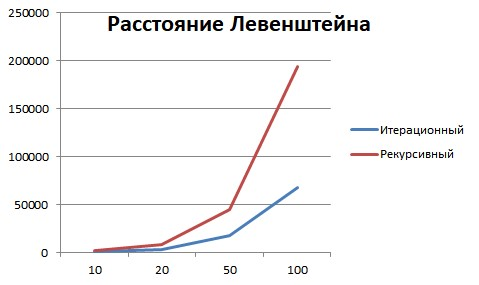
\includegraphics[scale=0.75]{img/levGraphic}
        \caption{График времени выполнения алгоритмов поиска расстояния Левенштейна}
        \label{fig:levGraphic}
    \end{figure}

    \begin{figure}[H]
        \centering
        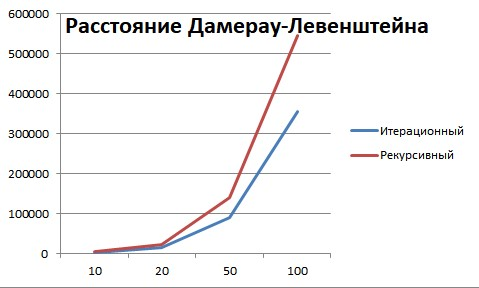
\includegraphics[scale=0.75]{img/levDamGraphic}
        \caption{График времени выполнения алгоритмов поиска расстояния Дамерау-Левенштейна}
        \label{fig:levDamGraphic}
    \end{figure}


    \section{Использование памяти}
    Алгоритмы нахождения расстояний Левенштейна и Дамерау-Левенштейна практически
    не отличаются друг от друга с точки зрения используемой памяти.

    Максимальная глубина стека вызовов при рекурсивной реализации --- сумма длин входных строк.
    Тогда максимальный объем требуемой памяти равен:

    \begin{equation}
        (len(Str_{1}) + len(Str_{2})) \cdot
        (2 \cdot K(String) + 7 \cdot K(int)),
    \end{equation}
    $len$ --- оператор вычисления длины строки,
    $Str_{1}$ и $Str_{2}$ --- входные строки,
    где $K$ --- оператор вычисления размера,
    $String$ --- строковый тип, $int$ --- целочисленный тип.

    Объем используемой памяти при итерационной реализации равен:
    \begin{equation}
        (len(Str_{1}) + 1) \cdot (len(Str_{2}) + 1) \cdot K(int) +
        4 \cdot K(int)
    \end{equation}


    \section{Вывод}
    Рекурсивные реализации алгоритмов нахождения расстояний Левенштейна и Дамерау-Левенштейна
    без использования матрицы работают дольше их итерационных реализаций.
    Время работы алгоритмов увеличивается в геометрической прогрессии.
    Рекурсивный алгоритм с использованием матрицы работает лишь немногим медленнее итерационного.

    \chapter*{Заключение}
    \addcontentsline{toc}{chapter}{Заключение}
    В ходе проделанной работы был изучен метод динамического программирования на материале реализации
    алгоритмов нахождения расстояний Левенштейна и Дамерау-Левенштейна.
    Были изучены алгоритмы поиска расстояний Левенштейна и Дамерау-Левенштейна и получены навыки
    реализации указанных алгоритмов в матричной и рекурсивных версиях,
    в том числе и с запоминанием результатов в матрицу.

    Экспериментально подтверждено различие во временной эффективности рекурсивной и итерационной
    реализаций алгоритмов поиска расстояний Левенштейна и Дамерау-Левенштейна
    при помощи разработанного программного обеспечения с замерами процессорного времени.
    Рекурсивные реализации проигрывают по времени в несколько раз.

    Теоретически было рассчитано использование памяти в каждой из реализаций алгоритмов поиска
    расстояний Левенштейна и Дамерау-Левенштейна. Рекурсивный алгоритм с использованием матрицы
    использует больше всего памяти.

    \newpage
    \addcontentsline{toc}{chapter}{Литература}

    \bibliographystyle{utf8gost705u}  % стилевой файл для оформления по ГОСТу
    \bibliography{report_1}          % имя библиографической базы (bib-файла)

\end{document}